\documentclass{article}
\usepackage[a4paper]{geometry}
\usepackage[spanish]{babel}
\usepackage{parskip}
\usepackage{setspace}
\usepackage{graphicx}
\usepackage{fancyhdr}
\usepackage{typearea}
\geometry{total={6in, 9in}}
\usepackage{blindtext} % no sé 
\usepackage{makeidx} % no sé 
\usepackage{lscape}
\usepackage{pdflscape}
\usepackage{fancyhdr}
\usepackage{pdfpages}
\usepackage{rotating}
\usepackage{etoolbox}
\usepackage[absolute]{textpos}


\newcommand{\tabitem}{%
  	\usebeamertemplate{itemize item}\hspace*{\labelsep}}
\usepackage[hidelinks]{hyperref}

%HEADRULE

\pagestyle{fancy}
\setlength{\headheight}{30.2pt}
\setlength{\headsep}{30pt}
% INICIO DE PÁGINAS
\begin{document}
\begin{titlepage}
	
	
	\begin{center}
		{\LARGE \textbf{UNIVERSIDAD NACIONAL DE INGENIERÍA}}\\
		\vspace{5 mm}
		{\large \textbf{Facultad de Ingeniería Industrial y de Sistemas}}\\
		\vspace{15.5 mm}
		\begin{figure}[h]
			\centering 
			
\includegraphics[width=0.45\textwidth]{images/CiberSecFIIS.png}
		\end{figure}
		\vspace{4 mm}	
		{\Large \textbf{Informes de exploración de vulnerabilidades en HTB} }\\
		\vspace{5 mm}
		
		\onehalfspacing  % Espaciamiento 1.5
		{\Large \textbf{``{\@De las máquinas: OpenAdmin, Fuse \\Magic, Remote }''} }\\
		
		\singlespacing  % Fin del espaciamiento 1.5
		
		\vspace{4 mm}	

		\vspace{20 mm}
		{\large \textbf{ELABORADO POR:} }\\
		\vspace{10 mm}
		\begin{center}
			\begin{minipage}{0.7\textwidth}
			  \begin{itemize}
				\item \Large Alfonso Suárez, Luis
				\item \Large Mottoccanche Tantaruna, Joseph
				\item \Large Chi Jon, Lau
			  \end{itemize}
			\end{minipage}
		  \end{center}

		\vspace{5 mm}	
	\end{center}

\end{titlepage}


\clearpage
\tableofcontents
\clearpage
% ----------------------------OPENADMIN-----------------------------------
\section{OpenAdmin}
\subsection{Reconocimiento}
\subsection{Escaneo de Vulnerabilidades}
\subsection{Enumeración}
\subsection{Explotación}
\subsection{Post Explotación}


\clearpage
% ----------------------------REMOTE-----------------------------------
\section{Remote}
\subsection{Reconocimiento}
Lo primero a hacer en este caso es un escaneo de nmap, para encontrar algunos puertos abiertos y servicios corriendo, en este caso se encontraron los puertos 21, 80 y 445 abiertos principalmente.

\begin{figure}[h]
	\center
	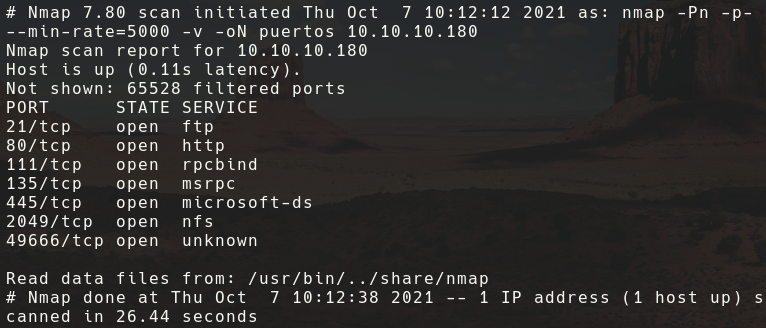
\includegraphics[width=0.8\textwidth]{images/remote/nmap_remote.png}
	\caption{nmap remote}
\end{figure}
 
\subsection{Escaneo de Vulnerabilidades}

Como primer escaneo de vulnerabilidades se intenta con el mismo nmap, con la opción "--script vuln", esto probará as vulnerabilidades más comunes en el server.

\begin{figure}[h]
	\center
	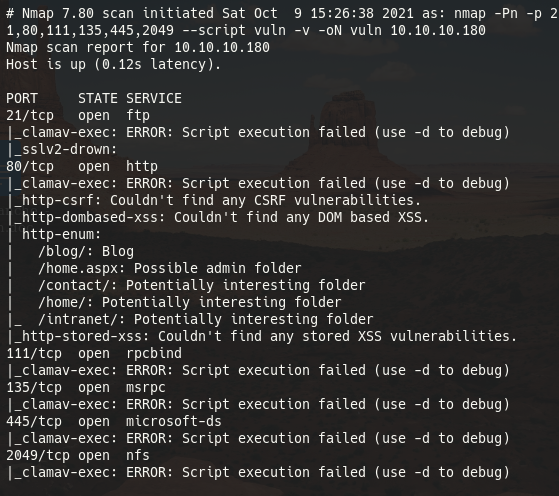
\includegraphics[width=0.7\textwidth]{images/remote/nmap_vuln.png}
	\caption{vulnerabilidades por nmap}
\end{figure}
\subsection{Enumeración}

Luego de ver los puertos, nmap no nos bota una vulnerabilidad por FTP, pero de todos modos nunca está de más probar si encontramos algo, sin embargo en esta ocasión no encontramos nada relevante.
\begin{figure}[h]
	\center 
	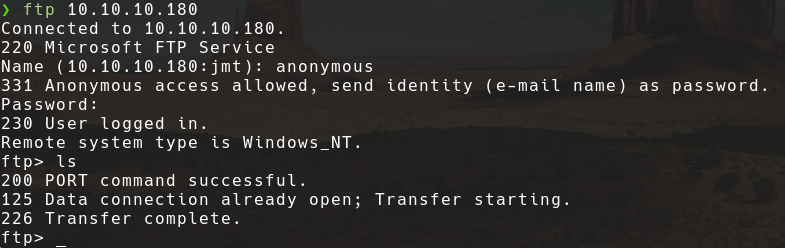
\includegraphics[width=0.8\textwidth]{images/remote/ftp.png}
	\caption{logueo anónimo por FTP}
\end{figure}

Intentamos luego con la página ubicada en el puerto 80, a ver si encontramos algo, y efectivamente encontramos una página que tiene diferentes apartados para revisar, buscamos info en los cuadros y en toda la página pero es solo texto generado de relleno, así que no hay información relevante en estas páginas para diccionarios.
\begin{figure}[h]
	\center 
	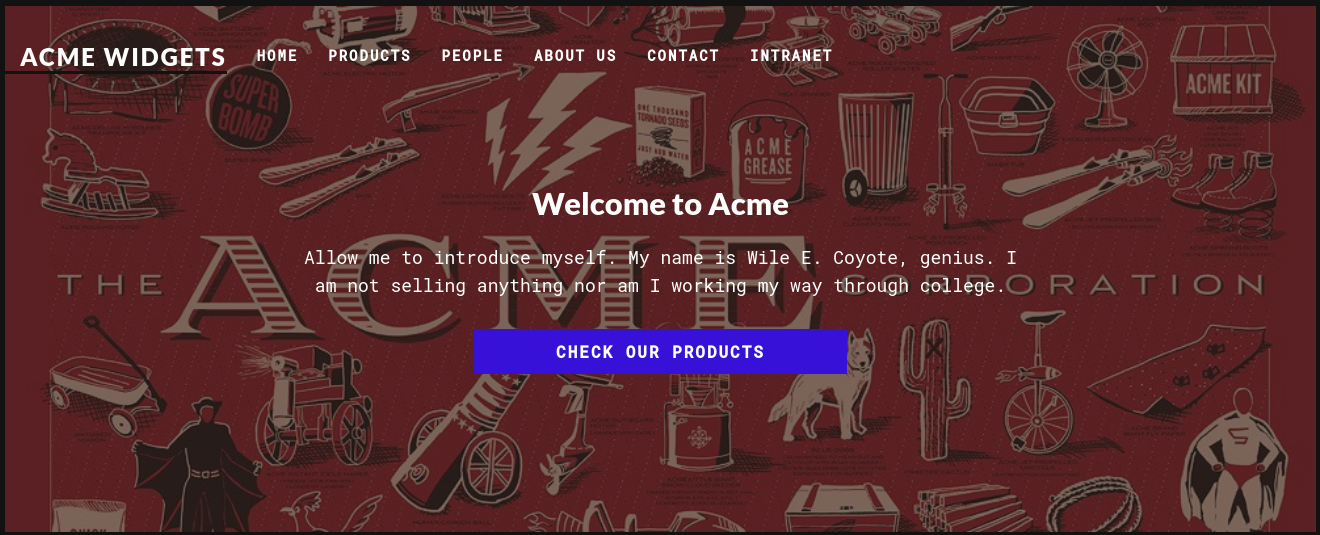
\includegraphics[width=0.8\textwidth]{images/remote/index_pagina.png}
	\caption{logueo anónimo por FTP}
\end{figure}

\clearpage

Entre todas las páginas encontramos un apartado de login, está en el mismo servidor así que se ve bastante interesante junto a que el framework es de umbraco según el wappalizer.
\begin{figure}[h]
	\center 
	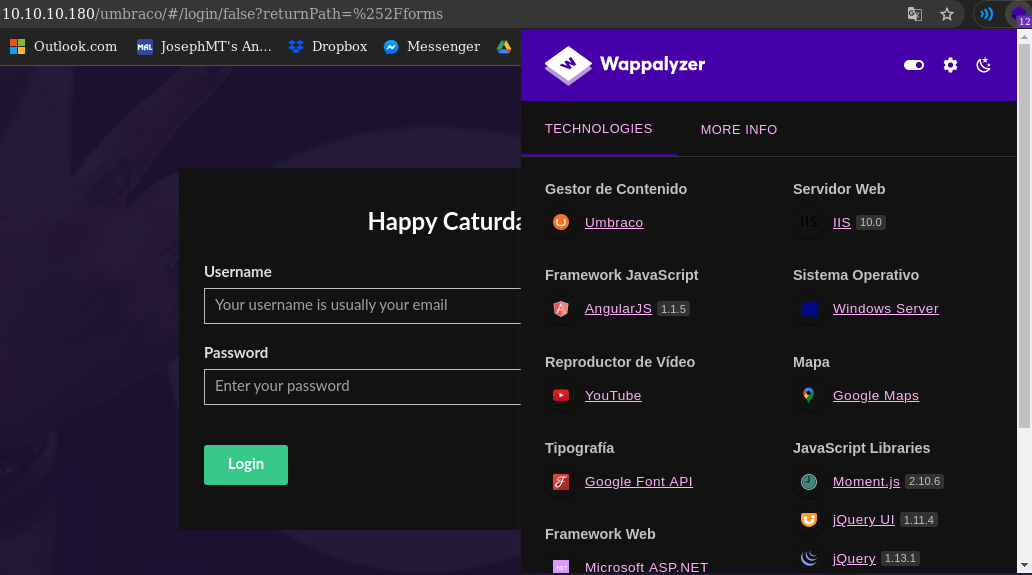
\includegraphics[width=0.8\textwidth]{images/remote/wappalizer.png}
	\caption{Resultados de wappalizer}
\end{figure}

Intentamos un escaneo con dirb para escanear los posibles directorios ocultos, donde se encontraron muchos directorios que de forma normal hubieran sido localizados y otros que hacen referencia a redirecciones, algunos que mostraron un error de configuración pero no grave.
\begin{figure}[h]
	\center 
	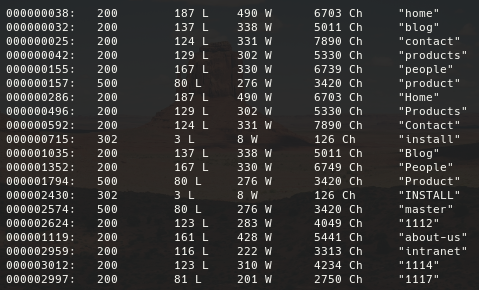
\includegraphics[width=0.8\textwidth]{images/remote/dirb.png}
	\caption{Escaneo con la herramienta dirb}
\end{figure}

\clearpage

Luego para tratar de buscar por los archivos compartidos se usa el comando llamado showmonts, que viene en la herramienta nfs-common.
\begin{figure}[h]
	\center 
	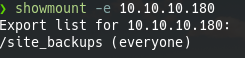
\includegraphics[width=0.6\textwidth]{images/remote/nfs.png}
	\caption{Obtención del backup}
\end{figure}

Luego creando una carpeta para guardar el contenido extraído con el comando "mount -t nfs 10.10.10.180:/site\_backups".
\\ una vez copiado esto tenemos carpetas interesantes, nuestro objetivo parecen ser credenciales de la base de datos para por medio de esas acceder al servidor original, entonces primero buscamos un poco.
\begin{figure}[h]
	\center 
	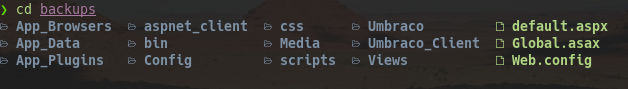
\includegraphics[width=0.8\textwidth]{images/remote/backup.png}
	\caption{Revisado del backup}
\end{figure}
Entonces encontramos una password en hash dentro de "App\_Data/Umbraco.sdf"
La obtuvimos mediante el comando strings probando en diferentes archivos de configuración grepeando pass, luego de encontrarla en esta ruta vimos que grepeando pass no nos daba mucha información adicional al correo de login, así que probamos otro filtro.
\begin{figure}[h]
	\center 
	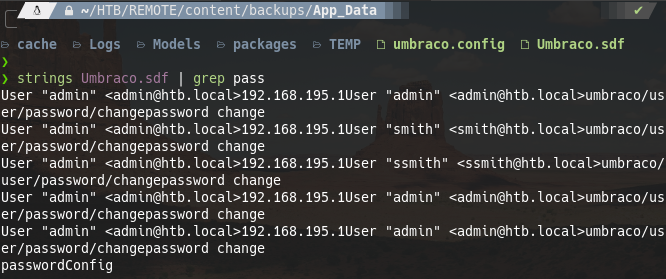
\includegraphics[width=0.8\textwidth]{images/remote/strings_pass.png}
	\caption{Encontrando el fichero con la contraseña}
\end{figure}

\clearpage

Entonces probando el filtro "admin" en base a los resultados anteriors, y encontramos un hash, el cual mediante hash-identifier pudimos comprobar su naturaleza SHA1.
\begin{figure}[h]
	\center 
	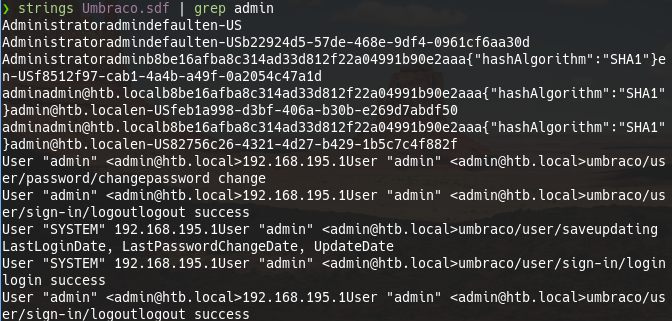
\includegraphics[width=0.8\textwidth]{images/remote/strings_admin.png}
	\caption{Encontrando la contraseña cifrada}
\end{figure}

Ahora posteriormente lo que sigue es intentar el crackeo de esta contraseña cifrada en SHA1, para nuestra suerte este tipo de cifrado es completamente obsoleto al poseer posiblidad de colisiones en su algoritmo.
Por lo cual en diferentes sitios online se pueden encontrar formas de crackear la contraseña, y el resultado es la obtención de la contraseña "baconandcheese".
\begin{figure}[h]
	\center 
	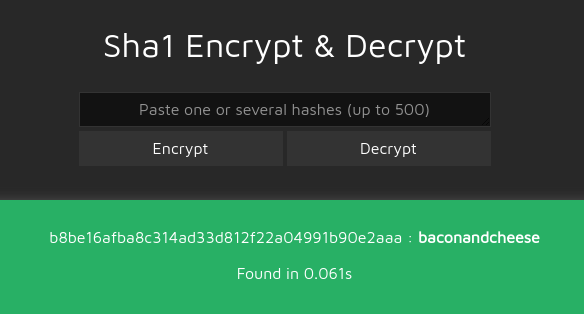
\includegraphics[width=0.8\textwidth]{images/remote/sha1.png}
	\caption{Encontrando la contraseña en texto claro}
\end{figure}

\clearpage

\subsection{Explotación}
\subsection{Post Explotación}

\clearpage
% ----------------------------FUSE-----------------------------------
\section{Fuse}
\subsection{Reconocimiento}
\subsection{Escaneo de Vulnerabilidades}
\subsection{Enumeración}
\subsection{Explotación}
\subsection{Post Explotación}

\end{document}
